\chapter{Daten Bereitstellung}

Wenn Daten von automatisierten Skripten untersucht werden sollen, können diese Daten unter Umständen nicht miteinander verglichen werden. Es spielt hierbei eine wichtige Rolle, dass alle Daten auf einem gleichen Stand sind, falls Zeitangaben eine Rolle spielen, sowie in einem gleichen Format gespeichert sind. Dies betrifft zum einen bereits vorhandene Daten, jedoch auch Daten, welche rein fiktiv erstellt wurden um spezielle Muster erkennen zu können. Im Folgenden werden die dazu verwendeten Methoden von Tobias Bloch genauer erklärt.


\section{Datenformat} \label{ch:format}

Da verschiedene Technologien während des Prozesses der Datenanalyse zum Einsatz kommen, muss ein einheitliches Format festgelegt werden, mit welchem die Daten gespeichert und weiter gegeben werden. Dabei waren die maßgeblichen Punkte, dass die Daten jederzeit von Menschen gelesen und überprüft werden können, sowie eine möglichst kompakte Speicherung. 

\needspace{6\baselineskip}
Das Format wurde daher auf eine CSV (Comma Separated Value) festgelegt. Dabei werden die einzelnen Daten hintereinander geschrieben und lediglich durch ein Komma (,) getrennt. Wie in \autoref{csvUnsorted} zu erkennen ist, kann auf den ersten Blick die Datenstruktur nachvollzogen werden. 

\needspace{6\baselineskip}
Bei den zu speichernden Daten handelt es sich um Binärdaten, welche nur zwei Zustände kennen: Funktionierend (0) und Störung (1). Dabei steht jedes Zeichen für einen Intervall, welchen wir standardmäßig auf eine Sekunde definiert haben.


\needspace{8\baselineskip}
\lstinputlisting[caption=Standard CSV mit Binär-Werten, label=csvUnsorted, breaklines=true]{dataPreparation/content/unsorted.csv}

\vspace{30pt}
\needspace{6\baselineskip}
Ein Problem an dieser Form tritt auf, wenn er sich um eine große Menge an Daten in einer Datei handelt. Bei zu vielen Zeilen verliert ein Mensch schnell den Überblick. Außerdem haben große Datenmengen einen hohen Speicherbedarf auf der Festplatte und kann Größen von 100 Megabyte erreichen.

\needspace{6\baselineskip}
Daher wurde das Format ein wenig abgeändert. Aufgrund der beschränkten Analyse, welche sich lediglich auf Binärdaten bezieht, kommen häufig Wiederholungen vor. Als Resultat werden aufeinander folgende Intervalle mit denselben Werten in einem Eintrag gespeichert. Dabei wird zuerst der Wert und nach einem Trennstrich die Anzahl der Wiederholungen angegeben. In \autoref{csvSorted} kann erkannt werden, dass selbst eine große Datenmenge von 8000 Intervallen einfach überblickt werden kann.


\needspace{8\baselineskip}
\lstinputlisting[caption=CSV mit gruppierten Binär-Werten, label=csvSorted, breaklines=true]{dataPreparation/content/TestDataShortSpikes.csv}

\newpage
\needspace{6\baselineskip}
Zusätzlich zu den gespeicherten Intervalldaten müssen auch allgemeine Informationen über den Inhalt der Datei gespeichert werden. Aus diesem Grund haben wir in der ersten Zeile einen \enquote{Header} mit allen dafür benötigten Informationen eingeführt. Zudem wird der Header durch das Dollarsymbol (\$) markiert, damit es beim maschinellen Auslesen leichter erfasst werden kann und nicht mit in die Auslese von Intervalldaten geraten kann.


\needspace{6\baselineskip}
In \autoref{csvHeader} ist der Header in einer Datei mit Maschinendaten enthalten. Die wichtigen Informationen sind, jeweils durch Komma getrennt, in vier sogenannten Key-Value-Paaren gespeichert. Das erste mit dem Namen \enquote{Machine} gibt den Namen der Maschine an, von welcher die Intervalle stammen. \enquote{Start} gibt den genauen Startpunkt des ersten Intervalls an, während \enquote{End} den letzten angibt. Unsere Dateien enthalten nur Werte von einem Tag, mehr dazu in \autoref{ch:transformation}. Unter \enquote{Intervall} wird der Abstand der einzelnen Intervalle in Millisekunden angegeben. Dieser Wert kann variiert werden und liegt im Standardfall bei einer Sekunde oder 1000 Millisekunden.

\vspace{60pt}
\needspace{4\baselineskip}
\lstinputlisting[caption=CSV mit Headereintrag, label=csvHeader, breaklines=true]{dataPreparation/content/BUP1FUE1_2015-07-22.csv}

\newpage
\needspace{6\baselineskip}
Für den Fall, dass zwei oder mehrere Intervallreihen miteinander verglichen werden sollen, können mehrere Reihen in einer Datei angegeben werden. Dabei gilt, dass ein Absatz den Beginn einer neuen Reihe einleitet. Wie in \autoref{csvMoreFiles} zu erkennen, enthält eine Zeile entweder einen Header, der für die darunter stehende Zeile Informationen enthält. Die Speicherung in einer Datei hilft bei einer gezielten Untersuchung der Intervall untereinander, da auf diese Weise besser nachvollzogen werden kann, welche Werte miteinander verglichen wurden.

\vspace{30pt}
\needspace{4\baselineskip}
\lstinputlisting[caption=CSV mit mehreren Intervallreihen, label=csvMoreFiles, breaklines=true]{dataPreparation/content/moreFiles.csv}


\vspace{20pt}
\needspace{6\baselineskip}
Die Erstellung einer Datei mit verschiedenen Daten geschieht nach aktuellem Stand nicht automatisch, sondern muss manuell ausgeführt werden. Ein Algorithmus zur Automatischen Untersuchung könnte in Zukunft angesetzt werden, wenn ein sinnvolles Vergleichsmuster ermittelt wurde. Unsere Untersuchung hat sich auf spezielle Vergleiche bezogen, weshalb manuelles Eingreifen gerechtfertigt war. 


\needspace{6\baselineskip}
Ein anderer Ansatz für die Speicherung der Intervalreihen hätte in einer Datenbank geschehen können. Dies hätte jedoch größeren Aufwand zur Folge und wäre problematisch beim Austausch der Daten untereinander gewesen. Da es im Umfang dieser Arbeit mit unserer Variante angemessen funktioniert hat, fanden wir den Einsatz einer Datenbank für unnötig.

\newpage
\section{Daten Generierung} \label{ch:generation}

Für die Analyse von Datenintervallen werden Testdaten benötigt, welche auf die verschiedenen Muster untersucht werden können. Aus diesem Zusammenhang wurde im Rahmen dieser Arbeit eine Anwendung programmiert, welche je nach Parameterangaben verschiedene Testdateien generieren kann. Dabei gilt, dass 0 der Normalzustand ist und 1 einen Problemzustand darstellt.

\needspace{6\baselineskip}
Bei dieser Anwendung handelt es sich um eine Konsolenapplikation, welche in C\texttt{\#} mit dem .NET Core Framework geschrieben wurde. Durch die Verwendung von .NET Core wird sichergestellt, dass das Programm neben Windows auch auf Mac und Linux mit vollem Umfang lauffähig ist. 

\needspace{6\baselineskip}
Der Benutzer gibt der Anwendung seine Einstellungen entweder über Kommandozeilenparameter (siehe Abbildung \autoref{fig:commando}) mit oder über die Konsolenanwendung, welche nach den nicht angegebenen Parametern frägt. Das Ergebnis wird in einer CSV-Datei in unserem Format (siehe \autoref{ch:format}) abgespeichert. Der Ablaufprozess wird in \autoref{fig:genUml} verdeutlicht.

\vspace{20pt}
\needspace{6\baselineskip}
\begin{figure}[tbph]
	\centering 
	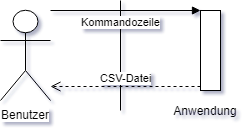
\includegraphics[width=0.6\textwidth,keepaspectratio] {dataPreparation/images/generationUml.png} 
	\caption{\label {fig:genUml} Use-Case-Diagramm der Generationsanwendung} 
\end{figure}


\vspace{20pt}
\needspace{6\baselineskip}
\begin{figure}[tbph]
	\centering 
	
\includegraphics[width=0.9\textwidth,keepaspectratio] {dataPreparation/images/commando.png} 
	\caption{\label {fig:commando} Aufruf des Programmes mit Kommandozeilenparameter} 
\end{figure}

\newpage
\needspace{8\baselineskip}
Als Parameter für die Anwendung gibt es verschieden Optionen, welche das Programm zum Start benötigt. Dabei handelt es sich um folgende:

\vspace{10pt}
\begin{description} 
	\item[IntervalsMaximum] \hfill \\ Integer, gibt die Anzahl der Intervalle an, welche generiert werden. Der Standartwert liegt hier bei 10000.
	\item[IsHighfrequent] \hfill \\ Nullable Boolean, kann die Generation beeinflussen, ob eher hochfrequente oder nieder frequente Sequenzen herauskommen. Kann auf null gesetzt werden um die Generation dem Zufall zu überlassen.
	\item[UsePattern] \hfill \\ Boolean, gibt an, ob bei der Generation willkürlich generiert werden soll oder bestimmte Muster (\enquote{Patterns}) genutzt werden sollen.
	\item[UseComplexRandom] \hfill \\ Boolean, der die Nutzung einer komplexeren Zufallsmethode angibt. Dies führt jedoch zu längeren Berechnungszeiten, weshalb er standardmäßig aus ist.
	\item[UseShortSaveForm] \hfill \\ Boolean, gibt an, ob die Kurzform des Speichersystemes genutzt werden soll (wie in \autoref{ch:format} beschrieben)
\end{description} 

\subsection{Algorithmus zur Datengenerierung}

Für die eigentliche Generierung der Daten wird ein Algorithmus verwendet, welcher im Zweck dieser Arbeit entstanden ist. Zuerst werden die mitgegebenen Parameter ausgelesen und analysiert. Dadurch können Optionen gesetzt werden, wie die maximale Länge eines Pattern (dt. Muster), die Häufigkeit von Patterns in der Sequenz und die möglichen Patterns.

\needspace{6\baselineskip}
Ein Pattern ist die Abfolge bestimmter 0 und 1 Kombinationen, welche wiederholt auftreten. Zwischen diesen Patterns befinden sich eine große Ansammlung von 0, da angenommen wird, dass die theoretische Maschine in diesen Zeiträumen ordnungsgemäß funktioniert. Durch den Parameter \enquote{IsHighfrequent} werden die Parameter auf die Frequenz beeinflusst, wodurch die Chance höher oder tiefer ist, dass entsprechende Frequenzen vorliegen.

\needspace{6\baselineskip}
Diese Patterns wurden im Zuge der Studienarbeit erstellt, damit eine Ähnlichkeit zwischen den generierten Intervallen und den maschinellen Daten besteht. Ein Pattern stellt hierbei eine gewisse Art von Problem dar, welche bei einer realen Maschine hätte auftreten können. Diese helfen zudem, dass in den computergenerierten Daten eine Form der Korrelation festgestellt werden kann, was bei zufällig generierten Daten nicht unbedingt gegeben wäre. 

\needspace{6\baselineskip}
Grundlegend geben die Patterns die Intervallmöglichkeiten an, welche bereits im vorangegangenen Kapitel erklärt wurden. Im Folgenden ist eine Liste aller möglichen Patterns:

\needspace{6\baselineskip}
\vspace{10pt}
\begin{description} 
	\item[Peak] \hfill \\ Einzelner Ausschlag von 1-5 Fehlerzuständen. Hierbei kann es sich um einen Messfehler oder ein kleines Problem handeln, welches sich sofort selbst behebt.
	\item[Block] \hfill \\ Langer Auschlag von 20-500 Fehlerzuständen. Symbolisiert ein größeres Problem, bei dem die Maschine stehen geblieben ist und nicht mehr funktioniert.
	\item[Shiver] \hfill \\ Schneller Wechsel von Funktionsfähigkeit und Fehlerzustand in 1-3er Abständen. Zeigt ein Problem, bei dem die Maschine mit Behinderung läuft.
	\item[Long Shiver] \hfill \\ Langsamer Wechsel von Funktionsfähigkeit und Fehlerzustand in 5-20er Abständen. Ähnlich dem normalen Shiver, aber mit mehr Abstand um die Variation zu erhöhen.
	\item[Random] \hfill \\ Zufallsgenerierte Ansammlung von 0 und 1. Stellt eine nicht sofort erklärbare Situation dar, welche mit geringer Wahrscheinlichkeit jederzeit auftreten kann.
\end{description}


\vspace{10pt}
\needspace{6\baselineskip}
Der grundsätzliche Algorithmus funktioniert in drei Einzelabschnitten. Zuerst wird die Anzahl der Patterns ermittelt, welche für die maximale Intervallänge angemessen sind. Die genaue Zahl ist zufällig, wird allerdings von der Option \enquote{IsHighfrequent} erhöht, falls diese gesetzt wurde. Durch die zufällige Anzahl an Patterns ergibt sich eine größere Vielfalt an unterschiedlichen Intervallen.

\needspace{6\baselineskip}
Sobald die Anzahl der Patterns klar ist, wird deren Länge und Abstand geklärt. Die Länge gibt die Anzahl an Werten an, die ein Intervall beinhaltet, während der Abstand die Anzahl von 0 zwischen zwei Patterns angibt. Diese Anzahlen werden ebenfalls zufällig generiert um Varianz zu schaffen.

\needspace{6\baselineskip}
Der letzte Schritt ist das Zuordnen der verschiedenen Patterns auf die entstandenen Patternplätze. Die Patterns werden zufällig ausgelost, allerdings mit unterschiedlicher Wahrscheinlichkeit. Dabei wird vor allem auf die Option \enquote{IsHighfrequent} Rücksicht genommen, wodurch viele Shiver und wenige Blöcke oder Peaks ausgewählt werden. 

\needspace{6\baselineskip}
Im Anschluss werden die Patterns mit entsprechender Länge und Abstand eingefüllt und das Intervall wird vollständig gebildet. Falls \enquote{UseShortSaveForm} gesetzt wurde, wird das Intervall auf die kurze Schreibweise aus \autoref{ch:format} umgewandelt. Das Ergebnis wird in einer CSV-Datei gespeichert.
\newpage
\section{Daten Transformation} \label{ch:transformation}

Nach der Untersuchung von simulierten Daten wurde auf reale Daten übergegangen. Dafür lagen uns Maschinendaten der Firma MPDV vor, welche über den Zeitraum 2016-2018 gesammelt wurden.

\needspace{6\baselineskip}
Wenn neben den simulierten Daten auch reale Daten untersucht werden sollen, dann müssen diese auf einen gemeinsamen Nenner gebracht werden, sodass die selben Methoden zur Untersuchung verwendet werden können. Daher lag der Entschluss nahe, die Maschinendaten der MPDV auf unser Format umzuwandeln.

\needspace{6\baselineskip}
Die Rohdaten wurden uns als CSV-Dateien gegeben, welche die Störmeldungen mehrerer Maschinen über mehrere Tage beinhalten. Als Ansatz wurde gewählt, ein Programm zu schreiben, welches die Rohdaten in unser Format umwandelt, wie es in \autoref{ch:format} beschrieben wurde. Hierfür wurde ebenfalls .NET Core verwendet, damit die Anwendung auf verschiedenen Betriebssystemen zum Einsatz kommen kann.

\needspace{6\baselineskip}
Bei einer Untersuchung der Rohdaten wurde klar, dass diese sehr viele Datensätze enthielt und relativ unübersichtlich aufgebaut war. Die Störmeldungen wurden einzeln aufgeführt, bei denen jeweils Start und Endzeit, sowie die entsprechende Meldung angegeben wurden. Die Zeiten sind jeweils in Sekunden angegeben und auf den gesamten Tag ausgelegt. Ein Ausschnitt wird in \autoref{csvRawdata} gezeigt. Bei dem jeweils ersten Ausdruck handelt es sich um den Maschinennamen, danach folgt Startzeit, Datum, Endzeit sowie die Störmeldung als Zahlencode.


\needspace{8\baselineskip}
\lstinputlisting[caption=CSV mit Rohdaten, label=csvRawdata, breaklines=true]{dataPreparation/content/rawdata.csv}


\needspace{6\baselineskip}
Die MPDV Dateien waren mit ihrer Größe bis zu 20 Megabyte relativ voll gepackt und mussten reduziert werden. Der Ansatz war, für jede Maschine und jeweils jeden Tag eine eigene Datei zu erstellen. Dies sollte die Möglichkeit verbessern gezielt dieselbe Maschine an unterschiedlichen Tagen oder verschiedene Maschinen miteinander zu vergleichen.

\needspace{6\baselineskip}
Die Konsolenanwendung zur Transformation ist relativ simpel aufgebaut und besitzt keinerlei Einstellungsmöglichkeiten. Als einziger Input ist der Pfad zu einer MPDV-Datei erforderlich. Der Algorithmus sortiert zuerst alle Einträge, welche in den Rohdaten zu finden sind. Dabei wird die Nutzung von Objektorientierter Programmierung genutzt. Ein Klassendiagramm ist unter \autoref{fig:transformationClass} zu sehen.

\vspace{20pt}
\needspace{6\baselineskip}
\begin{figure}[tbph]
	\centering 
	
\includegraphics[width=0.9\textwidth,keepaspectratio] {dataPreparation/images/transformationClass.png} 
	\caption{\label {fig:transformationClass} Klassendiagramm für die Datenspeicherung} 
\end{figure}

\vspace{15pt}

\needspace{6\baselineskip}
Für jede neue Maschine wird ein neues Objekt angelegt mit dem jeweiligen Maschinennamen. Für jeden Tag, an dem Daten für die entsprechende Maschine vorliegen, wird ein \enquote{Day}-Objekt mit dem entsprechenden Datum der Maschine hinzugefügt. In diesem Objekt werden alle Einträge an diesem Tag gespeichert. Diese strukturierte Speicherung ermöglicht eine bessere Übersicht und verbessert die Weiterverarbeitung der Daten im nächsten Schritt.

\needspace{6\baselineskip}
Da in dem unter \autoref{ch:format} definiertem Format die Statusmeldungen in Intervallen gespeichert sind, muss nun eine Transformation stattfinden. Deswegen werden für jeden Tag die Sekunden fortlaufend hochgezählt und auf vorliegende Störmeldungen überprüft. Dabei gilt, dass jede Störmeldung mit einer \enquote{1} gekennzeichnet wird und der Normalzustand mit \enquote{0}.

\needspace{6\baselineskip}
Jede dieser umgewandelten Tage wird danach in einer eigenen Datei gespeichert und mit einem entsprechenden Header versehen. Der Header ist in diesem Fall wichtig, da ansonsten die Hintergrunddaten, von welcher Maschine und welchem Tag die Daten stammen, verloren gehen würden. Diese Dateien können im Anschluss ausgewertet werden.
